\chapter{The Cosserat Theory of Elastic Rods} \label{chap:model}
%
In this chapter a system of equations which determine the configurations of a geometrically exact rod under a variety of (generalised) forces is introduced. The rod configurations are determined by the (generalised) strains of the system. The strains are related to the stresses on the rod by a set of constitutive relations, which when hyperelastic allow a variational formulation. A family of balance equations then describe the stresses on the rod. For a thorough exposition of rod theory see~\cite{Antman95}.
%
\section{Kinematic Equations} \label{sec:kinematic}
%
In this section the equations which define a Cosserat rod are introduced. A Cosserat rod is defined by a one-dimensional curve, called the centreline, along which a right-handed orthonormal triad, called the directors, are attached. The centreline describes the position of the rod while the directors describe the orientation of the cross section of the rod. The rod, $\boldsymbol{r}\left(s\right)$, is embedded in the spatial frame as the vector space spanned by the righthanded orthonormal triad of directors $\left\{ \, \boldsymbol{e}_{1}(s), \boldsymbol{e}_{2}(s), \boldsymbol{e}_{3}(s) \, \right\}$. The body frame, also referred to as the director frame, is given by a local rod-centred right-handed orthonormal triad $\left\{ \, \boldsymbol{d}_{1}(s), \boldsymbol{d}_{2}(s), \boldsymbol{d}_{3}(s) \, \right\}$. For clarity vectors in the spatial frame are denoted as $\boldsymbol{p}$ and components of the vector in the director frame form a 3-tuple denoted by the sans serif $\mathsf{p} = \left( \boldsymbol{p}\cdot \boldsymbol{d}_{1}, \boldsymbol{p}\cdot \boldsymbol{d}_{2}, \boldsymbol{p}\cdot \boldsymbol{d}_{3} \right)$. By orthonormality, the directors satisfy
%
\begin{subequations}
\label{eq:orthonormality}
\begin{align}
\boldsymbol{d}_{i}\left( s \right) \cdot \boldsymbol{d}_{j}\left( s \right) & = \delta_{ij}, \quad\quad i = 1,2,3 \quad j=1,2,3 \\
\boldsymbol{d}_{i}\left( s \right) \times \boldsymbol{d}_{j}\left( s \right) & =  \varepsilon_{ijk} \boldsymbol{d}_{k}\left( s \right)
\end{align}
\end{subequations}
%
\begin{figure}[!t] %
\label{fig:rod_diagram} %
\begin{center} %
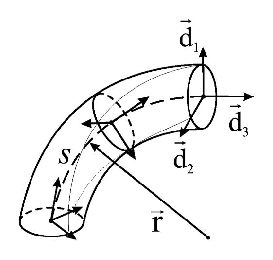
\includegraphics{Images/rod.eps} %
\caption[A Cosserat rod]{\baselineskip=1.0\normalbaselineskip%
Schematic diagram showing the orthornormality of the directors along the arclength.} %
\end{center} %
\end{figure} %
% 
where $\delta_{ij}$ is the Kronecker delta and $\varepsilon_{ijk}$ is the standard Levi-Civita permutation symbol. The orthogonality of the directors shall be exploited throughout the rod models derived. %
%
\par
Let $R$ be an element of the special orthogonal group, $SO\left(3\right)$, i.e. a smooth, left-acting, invertible transformation that converts quantities from the spatial frame into the director frame. Thus
%
\begin{align}
\boldsymbol{d}_{i} & = {R}\boldsymbol{e}_{i} \quad \mbox{for} \quad i = 1,2,3. 
\label{eq:frame}
\end{align}
%
The Lie group $SO\left(3\right)$ consists of the set of all three-by-three skew-symmetric matrices with unit determinant. An element of the corresponding Lie algebra $\mathfrak{so}\left(3\right)$ may be related to an element of $\mathbb{R}^{3}$ through the ``hat map'' isomorphism
%
\begin{equation}
a = \left( a_{1}, a_{2}, a_{3} \right) \in \mathbb{R}^{3} \quad \mbox{and} \quad \hat{a} \in \mathfrak{so}\left(3\right) \quad \mbox{with} \quad \hat{a} \cong 
\left( \begin{array}{ccc}
0 & -a_{3} & a_{2} \\
a_{3} & 0 & -a_{1} \\
-a_{2} & a_{1} & 0 
\end{array} \right) .
\label{eq:isomorphism}
\end{equation}
%
Thus for $\hat{a} \in \mathfrak{so}\left(3\right)$ and $b \in \mathbb{R}^{3}$ then $\hat{a}b = a \times b$.
%
\par
The evolution of the directors along the rod is found by differentiating equation~\eqref{eq:frame} in the spatial frame with respect to the parameter $s$
%
\begin{align}
\boldsymbol{d}^{\prime}_{i} & = {R}^{\prime}_{} \boldsymbol{e}_{i}^{} \nonumber \\
& = {R}^{\prime} {R}^{-T} \boldsymbol{d}_{i} \nonumber \\
& = \hat{\boldsymbol{u}} \boldsymbol{d}_{i} \nonumber \\
& = \boldsymbol{u} \times \boldsymbol{d}_{i} . 
\label{eq:directors}
\end{align}
%
Where $\hat{\boldsymbol{u}}:=R^{\prime}R^{-T}$ and $\boldsymbol{u}$ is defined to be a set of generalised strains. Thus, using the dot product and the orthogonality of the directors, the components of the strain $\boldsymbol{u}$ are expressed as
%
\begin{align}
u_{i}^{} & = \frac{1}{2} \varepsilon_{ijk}^{} \boldsymbol{d}^{\prime}_{j} \cdot \boldsymbol{d}_{k}^{}. \label{eq:curvatures}
\end{align}
%
The second set of strains $\boldsymbol{v}$ are defined as
%
\begin{align}
\boldsymbol{v} & = \boldsymbol{r}^{\prime}. 
\label{eq:centreline}
\end{align}
%
The triples ${\mathsf{u}} = \left( u_{1}, u_{2}, u_{3} \right)$ and ${\mathsf{v}} = \left( v_{1}, v_{2}, v_{3} \right)$ are the generalised strains in the body. Thus the projections onto the director frame $v_{1}=\boldsymbol{v}\cdot\boldsymbol{d}_{1}$ and $v_{2}=\boldsymbol{v}\cdot\boldsymbol{d}_{2}$ are associated with transverse shearing, while $v_{3}=\boldsymbol{v}\cdot\boldsymbol{d}_{3}$ is a measure of extension if positive and compression if negative. Likewise, $u_{1}=\boldsymbol{u}\cdot\boldsymbol{d}_{1}$ and $u_{2}=\boldsymbol{u}\cdot\boldsymbol{d}_{2}$ are associated with torsional bending and $u_{3}=\boldsymbol{u}\cdot\boldsymbol{d}_{3}$ is a measure of the twist in the body. Often the strain $u_{3}$ is referred to as the local twist and is denoted by $\tau=u_{3}$. Since it is natural to assume that rod cannot be compressed to zero length it is assumed
%
\begin{align}
v_{3} & > 0. \nonumber
\end{align}  
%
\par
If a rod is unshearable then
%
\begin{equation}
v_{1} =\boldsymbol{v} \cdot \boldsymbol{d}_{1} = 0 \quad \mbox{and} \quad v_{2} = \boldsymbol{v} \cdot \boldsymbol{d}_{2} = 0.\nonumber
\end{equation} 
%
If a rod is inextensible  
%
\begin{align*}
\left| \boldsymbol{r}^{\prime} \right| & = 1.
\end{align*}
%
Thus, the centreline of an unshearable and inextensible rod is determined by the single condition 
%
\begin{align}
\boldsymbol{r}^{\prime} & = \boldsymbol{d}_{3}
\label{eq:inextensible}
\end{align}
%
and parameter $s$ can now be interpreted as the arc-length of the rod.
%
\section{Constitutive Relationships} \label{sec:constitutive}
%
Having formulated the configurations of a Cosserat rod in terms of the strains $\boldsymbol{u}$ and $\boldsymbol{v}$, in this section the relationship between the stresses and the strains are introduced. 
%
\par
How the strains behave under stress determines the material properties of the rod and the constitutive relations relate the strains to the stresses. If the rod is hyperelastic then there exists a strain density function explicitly dependent on the generalised strains, i.e. $\mathcal{W}\left( \mathsf{u}-\mathsf{u}_{0},\mathsf{v}-\mathsf{v}_{0},s \right)$, such that the components of the force $\mathsf{n}=\left(n_{1},n_{2},n_{3}\right)$ and moment $\mathsf{m}=\left(m_{1},m_{2},m_{3}\right)$ in the body are 
%
\begin{equation}
m_{i} = \frac{\partial \mathcal{W}}{\partial u_{i}} \quad \mbox{and} \quad n_{i} = \frac{\partial \mathcal{W}}{\partial v_{i}},\label{eq:constit}
\end{equation}
%
where $\mathsf{u}_{0}$ and $\mathsf{v}_{0}$ are the strains associated with the unstressed rod. If the rod is uniform then the constitutive relations are the same throughout the rod 
%
\begin{align}
\mathcal{W}\left(\mathsf{u}-\mathsf{u}_{0},\mathsf{v}-\mathsf{v}_{0}\right) & = \mathcal{W}\left( \mathsf{u}-\mathsf{u}_{0},\mathsf{v}-\mathsf{v}_{0},s\right). \label{eq:nondegeneracy_1}
\end{align}
%
A hyperelastic rod will have a convex strain density function, that is the matrix of partial derivatives is positive definite
%
\begin{align}
\left|
\begin{array}{cc}
{\partial \mathsf{m}}\slash{\partial \mathsf{u}} & {\partial \mathsf{m}}\slash{\partial \mathsf{v}} \\
{\partial \mathsf{n}}\slash{\partial \mathsf{u}} & {\partial \mathsf{n}}\slash{\partial \mathsf{v}}
\end{array}
\right| & > 0. \label{eq:nondegeneracy_2}
\end{align}
%
Thus, an increase in the applied bending moment will accompany an increase in the bending strain. The hyperelastic strain function will also be coercive, that is
%
\begin{equation}
\dfrac{ \mathcal{W}\left(\mathsf{u}-\mathsf{u}_{0},\mathsf{v}-\mathsf{v}_{0}\right) }{ \sqrt{ \left|\mathsf{u}\right|^2 + \left|\mathsf{v}\right|^2} } \rightarrow \infty \quad \mbox{as} \quad \left|\mathsf{u}\right|^2 + \left|\mathsf{v}\right|^2 \rightarrow \infty. \label{eq:nondegeneracy_3}
\end{equation}
%
This implies that extremal values of the stresses must accompany extremal values of the strains. Finally, the strain energy density will have a nondegenerate minimum in the unstressed configuration 
%
\begin{align}
0 & = \left. \dfrac{\partial \mathcal{W}}{\partial \mathsf{u}} \right|_{\mathsf{u}=\mathsf{u}_{0},\,\mathsf{v}=\mathsf{v}_{0}} = \left.\dfrac{\partial \mathcal{W}}{\partial \mathsf{v}}\right|_{\mathsf{u}=\mathsf{u}_{0},\,\mathsf{v}=\mathsf{v}_{0}}. \label{eq:nondegeneracy_4}
\end{align}
%
The convexity of the hyperelastic strain-energy density function means that the strains can be inverted (locally) for the stresses, hence the hyperelastic function can be written as $\widetilde{\mathcal{W}}\left(\mathsf{m},\mathsf{n}\right)~\!=~\!\widetilde{\mathcal{W}}\left(\tilde{\mathsf{u}}\left({\mathsf{m}},{\mathsf{n}}\right),\tilde{\mathsf{v}}\left({\mathsf{m}},{\mathsf{n}}\right)\right)$. This assumption is crucial in that it allows the hyperelastic function to be related to the Hamiltonion via the Legendre transform. %
%
\par
An important property of many rod is isotropy. Assuming the material is transversally isotropic requires 
%
\begin{equation}
\tilde{\mathsf{u}}\left( Q \mathsf{m}, Q\mathsf{n}, s \right) = Q \tilde{\mathsf{u}}\left(\mathsf{m},\mathsf{n},s\right) \quad \mbox{and} \quad \tilde{\mathsf{v}}\left( Q \mathsf{m}, Q\mathsf{n}, s \right) = Q \tilde{\mathsf{v}}\left(\mathsf{m},\mathsf{n},s\right), \label{eq:isotropic}
\end{equation}
%
where $Q$ is a constant orthogonal matrix of the form 
%
\begin{align}
Q & = \left( 
\begin{array}{ccc}
Q_{11} & Q_{12} & 0 \\
Q_{21} & Q_{22} & 0 \\
0 & 0 & 1 
\end{array}
\right). \nonumber
\end{align}
%
It can be shown~\cite{Antman81} using Cauchy's Representation Theorem, that for nonlinear isotropic constitutive relationships the strain density function takes the arguments
%
\begin{align}
\widetilde{\mathcal{W}} & = \widetilde{\mathcal{W}}\left( m_{1}^{2} + m_{2}^{2}, m_{3}^{}, n_{1}^{2}+n_{2}^{2}, n_{3}^{}, m_{1}^{}n_{1}^{}+m_{2}^{}n_{2}^{}, m_{1}^{}n_{2}^{}-m_{2}^{}n_{1}^{}\right) .
\label{eq:constitutive_constraints}
\end{align}
%
\par
For an inextensible, unshearable rod the strain-density function for an initially straight and untwisted rod is a function of the strains ${\mathsf{u}}$ only, that is, $\mathsf{u}_{0} = \left(0,0,0\right)$ and $\mathsf{v} = \mathsf{v}_{0} = \left(0,0,1\right)$. In fact, for a rod under end tension and moment, nonlinear constitutive laws make little difference either in the underlying structure or the effective localised buckling modes for a rod under end tension and moment~\cite{Antman75,Champneys96b}. However, in order to separate nonlinear geometric effects from those caused by material nonlinearity, linear constitutive laws will be taken throughout. For simplicity, quadratic form, linear constitutive relationships, satisfying Hooke's law are chosen. The strain density function is given by 
%
\begin{align}
\mathcal{W} \left( {\mathsf{u}}, {\mathsf{v}} \right) & = \frac{1}{2}B_{1}\left(u_{1}+u_{0}\right)^{2} + \frac{1}{2}B_{2}u_{2}^{2} + \frac{1}{2} C u_{3}^{2} + \frac{1}{2} H v_{1}^{2} + \frac{1}{2} J {v_{2}^{2}} + \frac{1}{2} K v_{3}^{2}.
\label{eq:hyperelastic}
\end{align}
%
The constants $B_{1}=EI_{1}$, $B_{2}=EI_{2}$ and $C=GI_{3}$, where $I_{1}$ and $I_{2}$ are the principal moments of inertia about the $\boldsymbol{d}_{1}$ and $\boldsymbol{d}_{2}$ axes respectively, $I_{3}$ is the moment of inertia about the $\boldsymbol{d}_{3}$ axis, $E$ is Young's modulus and 
%
\begin{align}
G & = \frac{E}{2 \left(1+\nu\right)}\nonumber
\end{align} 
%
is the shear modulus, where $\nu$ is Poisson's ratio. The constants $H$ and $J$ are transverse shear stiffnesses and $K$ is the axial stiffness. The constant $u_{0}$ is a degree of initial curvature. It follows that $m_{1}$ and $m_{2}$ are associated with bending about the principal axes, $m_{3}$ with twist, $n_{1}$ and $n_{2}$ with shearing forces and $n_{3}$ with tension if positive, compression if negative. In the case of isotropy then $B_{1}=B_{2}$ and $H=J$.
%
\par
Having previously outlined how the rod configurations are determined by the strains and the relationships between strain and applied stress, in order to close the system it is now necessary to describe the structure of the applied stresses. 
%
\section{Equilibrium Equations} \label{sec:equilibrium}
%
In this section the static equilibrium balance equations are introduced. This is the final piece of information needed in order to construct the rod configuration. It shall be assumed that all forces and moments are suitable averages over the rod's cross section acting at the centreline of the rod. 
%
\subsection{Force-Free Rod} \label{subsec:twisted_equation}
%
In the spatial frame the equilibrium equation for a rod under constant end torque is
%
\begin{align}
\boldsymbol{m}^{\prime} & = \boldsymbol{0}.
\label{eq:fixed_frame}
\end{align}
% 
In the director frame the equation can be written as a non-canonical Hamiltonian system
%
\begin{align}
\mathsf{m}^{\prime} & = \mathcal{J}\left(\mathsf{m}\right) \nabla \mathcal{H}\left(\mathsf{m}\right),
\label{eq:noncan}
\end{align}
%
where the skew-symmetric structure matrix $\mathcal{J}= \mathcal{J}\left(\mathsf{m}\right)$ is given by
%
\begin{align}
\mathcal{J} & = -\mathcal{J}^{T} =
\left( 
\begin{array}{ccc}
0 & -m_{3} & m_{2} \\
m_{3} & 0 & -m_{1} \\
-m_{2} & m_{1} & 0 
\end{array} 
\right)
\label{eq:twist_structure}
\end{align}
%
and the Hamiltonian is
%
\begin{align}
\mathcal{H} & = \frac{1}{2} \mathsf{m} \cdot \mathsf{u}\left(\mathsf{m}\right) ,
\label{eq:twisted_hamiltonian}
\end{align}
%
with the strains as given in~\eqref{eq:constit}. For any two functions, $f$ and $g$ of $\mathsf{m}$, the Lie-Poisson bracket on the dual of the Lie algebra $\mathfrak{so}\left(3\right)$, corresponding to the structure matrix~\eqref{eq:twist_structure}, is given by
%
\begin{align}
\left\{ f , g \right\}_{\left(\mathsf{m}\right)} & = - \underbrace{ \mathsf{m} \cdot \left( \nabla_{\mathsf{m}}f \times \nabla_{\mathsf{m}} g \right) }_{\mbox{twist}}, 
\label{eq:twisted_bracket}
\end{align} 
%
where the Lie bracket is given by the direct sum of elements 
%
\begin{align}
\left[ {\xi}, {\eta} \right] & = \xi \times \eta \label{eq:direct_sum}
\end{align}
%
and the inner product is the dot product. Thus the governing equation~\eqref{eq:noncan} can be written as
%
\begin{align}
\mathsf{m}^{\prime} & = \left\{ \mathsf{m}, \mathcal{H}\right\}_{(\mathsf{m})} = \mathsf{m} \times \mathsf{u} . 
\label{eq:twisted}
\end{align}
%
\par
Note that when the constitutive relations are linear the Hamiltonian is quadratic and thus positive definite, hence the configurations are geodesic.
% 
\par
The null-space of the structure matrix~\eqref{eq:twist_structure} is one-dimensional and is spanned by the gradient of the Casimir
%
\begin{align}
\nabla C_{1} & = \frac{1}{2} \left( m_{1}, m_{2}, m_{3} \right)^{T} \nonumber
\end{align}
%
and hence
%
\begin{align}
C_{1} & = \mathsf{m} \cdot \mathsf{m}
\label{eq:twisted_casimir}
\end{align}
%
is a Casimir. The Casimir simply describes the fact that the magnitude of the total moment is constant along the rod. Since $\mathcal{H}$ is an integral, it follows from the Arnol'd-Liouville theorem~\ref{def:integrability} that~\eqref{eq:twisted} is completely integrable. In fact, the force-free rod is globally superintegrable~\cite{Fasso96,Fasso05,Hanssmann05}.
%
\par
Having introduced the Lie-Poisson bracket for the equilibrium equations, the strains can be computed from the constitutive relations and the centreline of the rod can then be recovered. In most practical applications however the boundary conditions will feature conditions on the orientation of the rod. The evolution of the fixed vectors in the director frame can be incorporated into the Lie-Poisson framework as a semidirect extension to the existing bracket. Thus, the evolution of centreline can be recovered from the field variables. The complete set of equations are 
%
\begin{align}
\left\{ f, g \right\}_{\left(\mathsf{m},\mathsf{e}_{1},\mathsf{e}_{2},\mathsf{e}_{3}\right)} & = \mathsf{m} \cdot \left( \nabla_{\mathsf{m}}f \times \nabla_{\mathsf{m}} g \right) + \mathsf{e}_{1} \cdot \left( \nabla_{\mathsf{m}}f \times \nabla_{\mathsf{e}_{1}} g + \nabla_{\mathsf{e}_{1}}f \times \nabla_{\mathsf{m}} g\right) \nonumber \\
& \hspace{2.0cm} + \mathsf{e}_{2} \cdot \left( \nabla_{\mathsf{m}}f \times \nabla_{\mathsf{e}_{2}} g + \nabla_{\mathsf{e}_{2}}f \times \nabla_{\mathsf{m}} g\right) \nonumber \\
& \hspace{2.5cm} + \mathsf{e}_{3} \cdot \left( \nabla_{\mathsf{m}}f \times \nabla_{\mathsf{e}_{3}} g + \nabla_{\mathsf{e}_{3}}f \times \nabla_{\mathsf{m}} g\right) \nonumber 
\nonumber
\end{align}
%
The extended Lie algebra is now given by $\mathfrak{so}\left(3,3\right) = \mathfrak{so}\left(3\right) \oplus_{s}\left( \mathbb{R}^{3} \times \mathbb{R}^{3} \times \mathbb{R}^{3}\right)$ but as the Hamiltonian is indepedent of the spatial frame the extensions to the bracket do not effect the configurations of the rod.
%  
\subsection{Kirchhoff Rod} \label{subsec:kirchhoff_equation}
%
The equilibrium equations for a rod under end tension and moment are given by
%
\begin{equation}
\boldsymbol{m}^{\prime} + \boldsymbol{r}^{\prime} \times \boldsymbol{n}=\boldsymbol{0} \quad \mbox{and} \quad \boldsymbol{n}^{\prime} = \boldsymbol{0}. 
\label{eq:kirchhoff_external}
\end{equation}
%
In the director frame the equations can be written in Hamiltonian form as
%
\begin{align}
\left( 
\begin{array}{c}
\mathsf{m} \\
\mathsf{n} 
\end{array}
\right)^{\prime} & = 
\mathcal{J}\left(\mathsf{m}, \mathsf{n}\right) \nabla \mathcal{H}\left( \mathsf{m}, \mathsf{n}\right),
\end{align}
%
where the structure matrix $\mathcal{J} = \mathcal{J}\left(\mathsf{m},\mathsf{n}\right)$ is given by
%
\begin{align}
\mathcal{J} & = -\mathcal{J}^{T} = 
\left( \begin{array}{cc} 
\hat{\mathsf{m}} & \hat{\mathsf{n}} \\
\hat{\mathsf{n}} & 0 
\end{array}
\right)
\label{eq:kirchhoff_structure}
\end{align}
%
and the Hamiltonian is now
%
\begin{align}
\mathcal{H} & = \frac{1}{2}\mathsf{m}\cdot\mathsf{u}\left(\mathsf{m},\mathsf{n}\right) +  \frac{1}{2}\mathsf{n}\cdot\mathsf{v}\left(\mathsf{m},\mathsf{n}\right). 
\label{eq:kirchhoff_hamiltonian}
\end{align}
% 
Thus the additional term can be considered to be the kinetic energy-density due to the end force.  The governing equations are
%
\begin{subequations}
\label{eq:kirchhoff}
\begin{align}
\mathsf{m}^{\prime} & = \left\{\mathsf{m}, \mathcal{H} \right\}_{(\mathsf{m},\mathsf{n})} = \mathsf{m} \times \mathsf{u} + \mathsf{n} \times \mathsf{v}, \label{eq:kirchhoff_moment} \\
\mathsf{n}^{\prime} & = \left\{\mathsf{n}, \mathcal{H} \right\}_{(\mathsf{m},\mathsf{n})} = \mathsf{n} \times \mathsf{u}  \label{eq:kirchhoff_force}.
\end{align}
\end{subequations}
%
which are the Lie-Poisson equations on the Cartesian pairing $\left( \mathsf{m}, \mathsf{n} \right)$ given by the bracket
%
\begin{align}
\left\{ f , g \right\}_{\left({\mathsf{m}},{\mathsf{n}}\right)} & = - \mathsf{m} \cdot \left( \nabla_{\mathsf{m}}f \times \nabla_{\mathsf{m}} g \right) - \underbrace{ \mathsf{n} \cdot \left( \nabla_{\mathsf{m}}f \times \nabla_{\mathsf{n}} g + \nabla_{\mathsf{n}}f \times \nabla_{\mathsf{m}} g\right) }_{\mbox{force}}.
\label{eq:kirchhoff_bracket}
\end{align}
%
An extra semidirect term, corresponding to the effect of the end force has been added when compared to the previous Lie-Poisson bracket~\eqref{eq:twisted_bracket}. Again the inner product is dot product but the Lie algebra now has the bracket 
%
\begin{align}
\left[ \left( \xi, u \right), \left( \eta, v\right) \right] & = \left( \xi\times\eta, \xi \times v - \eta \times u \right) .
\end{align}
%
Where $\left(\xi,u\right) \in \mathfrak{g}$. The Lie algebra is then given by $\mathfrak{g} = \mathfrak{so}\left(3,1\right) = \mathfrak{so}\left(3\right)\oplus_{s}\mathbb{R}^{3}$ and the moment $\mathsf{m}$ spans $\mathfrak{so}\left(3\right)$ and the force $\mathsf{n}$ spans $\mathbb{R}^{3}$. The associated Lie group now corresponds to the group of rotations and translations in~$\mathbb{R}^{3}$. As shall be shown in chapter~\ref{chap:reduction} knowledge of the underlying group is extremely helpful when reducing the system. 
%
\par
The additional term in the Hamiltonian, due to the end force, breaks the full $SO\left(3\right)$ symmetry. The equations~\eqref{eq:kirchhoff} are those for the motion of a heavy top when the rod is unshearable and inextensible.
% 
\par
The null-space of the structure matrix is two-dimensional and spanned by
%
\begin{equation}
\nabla C_{1} = \left(\begin{array}{c} \mathsf{n} \\ \mathsf{m} \end{array} \right) \quad \mbox{and} \quad \nabla C_{2} = \frac{1}{2} \left(\begin{array}{c} \mathsf{0} \\ \mathsf{n} \end{array} \right). \nonumber
\end{equation}
%
Hence the Casimirs are 
%
\begin{subequations}
\label{eq:kirchoff_casimirs}
\begin{align}
C_{1} & = \mathsf{n} \cdot \mathsf{m} \label{eq:kirchhoff_casimir1}, \\
C_{2} & = \mathsf{n} \cdot \mathsf{n} \label{eq:kirchhoff_casimir2}.\
\end{align} 
\end{subequations}
%
The Casimir~\eqref{eq:kirchhoff_casimir1} describes the conservation of the moment about the force vector, while~\eqref{eq:kirchhoff_casimir2} describes the conservation of the magnitude of force in the rod. 
%
\par
In addition to the Hamiltonian and the two Casimirs, a single first integral is required if the system is to be completely integrable.  There are two cases, both well-documented:
%
\begin{description}
\item[The Lagrange case] has an integral given by
\begin{align}
I_{1} &= \mathsf{m} \cdot \mathsf{d}_3 \quad \mbox{if} \quad B_{1} = B_{2} = B. \label{eq:lagrange}
\end{align}
Thus, if the two bending stiffnesses are equal then the (local) twist $m_3$ is a conserved quantity. For the Kirchhoff equation if the rod satisfies~\eqref{eq:isotropic} then the Lagrange integral holds for arbitrary nonlinear constitutive relationships. 
\item[The Kovalevskaya case] has an integral given by
\begin{align}
I_{1} & = \left( B_{1}^{2}m_{1}^{2} - C^{2} m_{3}^{2} + n_{3} \right)^{2} 
+ \left( 2 B_{1}^{} C m_{1}m_{3} - n_{1} \right)^{2} \quad \mbox{if} \quad B_{1} = C = 2B_{2}.
\label{eq:kov}
\end{align}
% 
Kovalevskaya found this integral by looking for the absence of certain types of singularities in complex time. Unlike the Lagrange integral the integral does not seem to have a clear physical interpretation.\footnote{Kovalevskaya won the Bordin Prize given by the Paris Academy of Sciences in 1886 and was considered such a achievement that the prize money was doubled.}
%
\par  
The condition on the bending stiffnesses renders the Kovalevskaya rod somewhat unphysical since it corresponds to a negative Poisson ratio. However, novel materials with negative effective Poisson ratio are now known. For instance, experimental measurements of bending and torsional stiffnesses of DNA molecules have led to the generally accepted range $0.7<K/K_3<1.5$~\cite{Schlick95}. It is unknown how nonlinear constitutive relations or properties such as shear and extensibility effect the Kovalevskaya integral.
\end{description}
%
There is another case which is not completely integrable on the entire phase space but is completely integrable on a single symplectic leaf.
%
\begin{description}
\item[The Chaplygin-Goryachev case] requires that the initial conditions must satisfy
\begin{align}
\mathsf{m} \cdot \mathsf{n} & = \mathsf{0} \nonumber
\end{align}
then the integral
\begin{align}
I_{1} = B_{2}^{} m_{2} \left( B_{1}^{2} m_{1}^{2} + B_{2}^{2}m_{2}^{2} \right) - C m_{3} n_{2} \quad \mbox{if} \quad B_{1} = 4 B_{2} = C \label{eq:chaplygin}
\end{align}
renders the system integrable. Similarly to the Kovalevskaya integral, this case relies on linear stress-strain relationships and it is unknown whether a corresponding integral exist for nonlinear constitutive relations. The only natural interpretation of the condition on the Casimir is to not apply end moment and then the Chaplygin-Goryachev case can be considered an anisotropic case of the elastica.  
\end{description}
%
It is simple to show that all the integrals~\eqref{eq:kirchoff_casimirs},~\eqref{eq:kirchhoff_hamiltonian} and either~\eqref{eq:lagrange},~\eqref{eq:kov}, or~\eqref{eq:chaplygin} are in involution with respect to the bracket~\eqref{eq:kirchhoff_bracket} and that generically integrable configurations exist on three-tori.
%
\subsection{An Elastic Conducting Rod in a Uniform Magnetic Field}\label{subsec:magnetic_equation}
%
Now consider a rod placed in a uniform magnetic field $\bar{\boldsymbol{B}}$. The rod carries a uniform current $\boldsymbol{I}=I\boldsymbol{r}^{\prime}$ of strength $I$ along the centreline, assuming the rod to be sufficiently slender for eddy currents within the cross section to be ignorable. The rod then experiences a Lorentz body force 
% 
\begin{align}
\boldsymbol{n}^{\prime} + \boldsymbol{F}_{L} & = \boldsymbol{0} \quad \mbox{where} \quad \boldsymbol{F}_L=\boldsymbol{I}\times\bar{\boldsymbol{B}} = I\boldsymbol{r}^{\prime}\times\bar{\boldsymbol{B}} = I\boldsymbol{v}\times\bar{\boldsymbol{B}}. 
\end{align}
% 
Let $\boldsymbol{B}=I\bar{\boldsymbol{B}}$ and let the magnetic field be aligned along the fixed axis $\boldsymbol{e}_{3}$ so that the equilibrium equations take the form
%
\begin{align}
\boldsymbol{m}^{\prime} + \boldsymbol{r}^{\prime} \times \boldsymbol{n}=\boldsymbol{0},  \quad  \boldsymbol{n}^{\prime} +  \boldsymbol{r}^{\prime} \times \boldsymbol{B}=\boldsymbol{0} \quad \mbox{and} \quad \boldsymbol{B}^{\prime} = \boldsymbol{0}.
\label{eq:magnetic}
\end{align}
%
It is necessary to assume that the current in the rod is moderate so that the effect of the magnetic field generated by the current is negligible compared to the external magnetic field.  
%
\par
In the director frame the governing equation is a non-canonical Hamiltonian system of the form
%
\begin{align}
\left(
\begin{array}{c}
\mathsf{m} \\
\mathsf{n} \\
\mathsf{B}
\end{array}
\right)^{\prime} & =
\mathcal{J} \left({\mathsf{m}},{\mathsf{n}},\mathsf{B}\right) \nabla \mathcal{H}\left({\mathsf{m}},{\mathsf{n}} \right),
\label{eq:noncanonical_structure}
\end{align}
%
where the structure matrix $\mathcal{J}=\mathcal{J} \left( \mathsf{m}, \mathsf{n}, \mathsf{B} \right)$ is given by
%
\begin{align}
\mathcal{J} = -\mathcal{J}^{T} & = \left( 
\begin{array}{ccc}
\hat{\mathsf{m}} & \hat{\mathsf{n}} & \hat{\mathsf{B}} \\
\hat{\mathsf{n}} & \hat{\mathsf{B}} & \mathsf{0} \\
\hat{\mathsf{B}} & \mathsf{0} & {\mathsf{0}}  
\end{array}
\right)
\label{eq:magnetic_structure}
\end{align}
%
and the Hamiltonian, once again, is 
%
\begin{align}
\mathcal{H} & = \frac{1}{2} \mathsf{m} \cdot \mathsf{u} + \mathsf{n}\cdot\mathsf{v}. \label{eq:magnetic_ham}
\end{align}
%
Note that the Hamiltonian is a function of $\mathsf{m}$ and $\mathsf{n}$ only, but the gradient is taken with respect to the three field variables. The Hamiltonian is the same as for the Kirchhoff rod: the effect of the magnetic field is only present in the structure matrix.  The governing equations can be written as
%
\begin{subequations}
\label{eq:magnetic_equations}
\begin{align}
\mathsf{m}^{\prime} & = \left\{\mathsf{m}, \mathcal{H} \right\}_{\left({\mathsf{m}},{\mathsf{n}}, {\mathsf{B}} \right)} = \mathsf{m}\times\mathsf{u} + \mathsf{n}\times\mathsf{v}, \label{eq:magnetic_moment} \\
\mathsf{n}^{\prime} & = \left\{\mathsf{n}, \mathcal{H} \right\}_{\left({\mathsf{m}},{\mathsf{n}}, {\mathsf{B}} \right)} = \mathsf{n}\times\mathsf{u} + \mathsf{B}\times\mathsf{v}, \label{eq:magnetic_force} \\
\mathsf{B}^{\prime} & = \left\{\mathsf{B}, \mathcal{H} \right\}_{\left({\mathsf{m}},{\mathsf{n}}, {\mathsf{B}} \right)} = \mathsf{B}\times\mathsf{u}, \label{eq:magnetic_vector}
\end{align}
\end{subequations}
%
where the Lie-Poisson bracket on $\left( \mathsf{m}, \mathsf{n}, \mathsf{B} \right)$ given by
%
\begin{align}
\left\{ f,g \right\}_{\left({\mathsf{m}},{\mathsf{n}}, {\mathsf{B}} \right)} & =
- {\mathsf{m}}\cdot\left(\nabla_{{\mathsf{m}}}f \times \nabla_{{\mathsf{m}}}g \right) 
- {\mathsf{n}}\cdot\left(\nabla_{{\mathsf{m}}}f \times \nabla_{{\mathsf{n}}}g + \nabla_{{\mathsf{n}}}f \times \nabla_{{\mathsf{m}}}g\right) \nonumber \\
& \hspace{1.25cm} - \underbrace{{\mathsf{B}} \cdot \left(\nabla_{\mathsf{m}}f \times \nabla_{\mathsf{B}}g +
\nabla_{\mathsf{B}}f \times \nabla_{{\mathsf{m}}}g \right)}_{\mbox{evolution of field}}
- \underbrace{\mathsf{B} \cdot \left( \nabla_{\mathsf{n}}f \times \nabla_{\mathsf{n}}g \right)}_{\mbox{effect of field}},
\label{eq:magnetic_bracket}
\end{align}
%
has been extended from the previous bracket by the addition of two more terms. The first term, a semidirect extension, describes the evolution of the magnetic field in the director frame and does not affect the force and moment balance since the Hamiltonian is independent of $\mathsf{B}$. The second term, called a Liebniz extension~\cite{Thiffeault00}, contains the Lorentz force. This term makes the bracket extension non-semidirect.  %
%
\begin{rem}
In the language of Lie algebra cohomology the bracket is extended by a semidirect and a Liebniz extensions. Cohomology studies the connections between the topology of the Lie group and the algebraic structure of the associated Lie algebra. Cohomology gives a class of linear transformations that preserve the structure of the normal forms of the bracket extensions. The parts of the extensions that are removed by such transformations are called coboundaries, those that remain are called cocycles. Cocycles are bilinear skew-symmetric functions on the Lie algebra which satisfy Jacobi's identity~\cite[pg.~372]{Arnold89}. The Liebniz extension is a cocycle and as the Hamiltonian is independent of the spatial frame, the semidirect extension is a coboundary. %
\end{rem}
% 
\par
The bracket which generates the Lie algebra is given by
%
\begin{align}
\left[ \left( \xi, u, w \right), \left( \eta, v, x \right) \right] & = \left( \xi\times\eta, \, \xi \times v - \eta \times u, \, \xi \times w - \eta \times x -  u \times v \right).\label{eq:bracket3}
\end{align}
%
Even though the nontrivial extension is of the simplest possible form~\cite{Thiffeault00} it leads to highly nontrivial generalisations of the symmetry groups. The Lie algebra includes $\mathfrak{so}\left(3\right)$ and $\mathbb{R}^{3}$ as proper subalgebras but is not purely composed of the semi-direct sum of the subalgebras. %
% 
\par
There are three Casimirs, given by
%
\begin{subequations}
\label{eq:magnetic_casimirs}
\begin{align}
C_{1} & = \frac{1}{2}\mathsf{n} \cdot \mathsf{n} + \mathsf{m} \cdot \mathsf{B}, \label{eq:magnetic_casimirs1} \\
C_{2} & = \mathsf{B} \cdot \mathsf{n}, \label{eq:magnetic_casimirs2} \\
C_{3} & = \mathsf{B} \cdot \mathsf{B}. \label{eq:magnetic_casimirs3}
\end{align} 
\end{subequations}
%
The magnitude of the magnetic force is conserved, thus~\eqref{eq:magnetic_casimirs3}. The magnitude of force is no longer conserved, but as a result of rotational symmetry the force component in the direction of the magnetic field is conserved resulting in~\eqref{eq:magnetic_casimirs2}. Casimir~\eqref{eq:magnetic_casimirs1} however does not seem to have a physical interpretation; it states that half the magnitude of the force in the body plus the moment about the direction of the magnetic field is a conserved quantity. %
%
\par
In the linearly elastic~\eqref{eq:hyperelastic}, unshearable, inextensible and isotropic case, that is $J=H=K=0$ and $B=B_1=B_2$, then two integrals emerge
%
\begin{subequations}
\label{eq:magnetic_integrals}
\begin{align}
I_{1} & = \mathsf{m}\cdot\mathsf{d}_3, \label{eq:magnetic_lagrange} \\
I_{2} & = \mathsf{n}\cdot\mathsf{m} + B \mathsf{B} \cdot \mathsf{d}_{3}. \label{eq:int2}
\end{align}
\end{subequations}
%
As in the Lagrange case the first of these integrals expresses the conservation of twist in the rod. The second integral, like the Kovalevskaya integral, does not seem to have a physical interpretation. The Lagrange integrability condition $B_1=B_2$ is unaltered by the magnetic field, but now there are additional requirements on constitutive relations in the form of linear elasticity, inextensibilty and shearability. Numerical evidence presented in~\cite{Thiffeault01} in the form of chaotic orbits suggests that the linearly elastic, inextensible, unshearable the magnetic rod with $B_1=C=2B_{2}$ is not integrable. Of course, a perturbed condition on the stiffnesses may exist for which the system is integrable. %
%
\par
It is a straightforward task to check that all the integrals~\eqref{eq:magnetic_ham},~\eqref{eq:magnetic_lagrange} and~\eqref{eq:int2} are independent and in involution with respect to the Lie-Poisson bracket~\eqref{eq:magnetic_bracket}. Hence in the isotropic case the system is completely integrable in the sense of Liouville and configurations lie on five-tori defined by two Casimirs, two integrals and the Hamiltonian. %
% 
\par
Note that due to the complexities of the Lie algebra, the Lie group which generates the Lie algebra is not known. That the underlying Lie group is not known means that a suitable parameterisation can not be constructed which gives a complete representation of the symmetries and hence integrals. Thus, presently, the system can not be reduced to a single degree of freedom canonical Hamiltonian system. %
%
\subsection{An Elastic Conducting Rod in a Nonuniform Magnetic Field} \label{subsec:twisted_field}
%
By inspection of the structure matrices~\eqref{eq:twist_structure},~\eqref{eq:kirchhoff_structure} and~\eqref{eq:magnetic_structure} it is natural to consider the system
%
\begin{align}
\boldsymbol{m}^{\prime} + \boldsymbol{r}^{\prime}\times\boldsymbol{n} = \boldsymbol{0}, \quad \boldsymbol{n}^{\prime} + \boldsymbol{r}^{\prime}\times\boldsymbol{B}=\boldsymbol{0}, \quad \boldsymbol{B}^{\prime} + \boldsymbol{r}^{\prime}\times\boldsymbol{D}=\boldsymbol{0} \quad \mbox{and} \quad \boldsymbol{D}^{\prime} = \boldsymbol{0}.
\label{eq:nonuniform_vec}
\end{align}
%
The equation for $\boldsymbol{B}$ can be integrated to give $B_x=y$, $B_y=-x$, $B_z=0$, where $x,y,z$ and $B_x,B_y,B_z$ are components of $\boldsymbol{r}$ and $\boldsymbol{B}$ relative to the fixed frame $\{\boldsymbol{e}_1,\boldsymbol{e}_2,\boldsymbol{e}_3\}$, and $\boldsymbol{e}_3$ is choosen to be in the direction of $\boldsymbol{D}$. Thus~\eqref{eq:nonuniform_vec} can be thought of as describing a rod in a linearly-varying magnetic field generated by a uniform `hypermagnetic' field $\boldsymbol{D}$. %
%
\par
In the director frame the equations take the Hamiltonian form
%
\begin{align}
\left( \begin{array}{cccc} 
\mathsf{m} \\
\mathsf{n} \\
\mathsf{B} \\
\mathsf{D}
\end{array} \right)^{\prime} & = \mathcal{J}\left( \mathsf{m}, \mathsf{n}, \mathsf{B}, \mathsf{D} \right) \nabla \mathcal{H}\left( \mathsf{m},\mathsf{n}\right), \quad \mbox{with} \quad \mathcal{H}\left(\mathsf{m},\mathsf{n}\right) = \frac{1}{2}\mathsf{m}\cdot\mathsf{u} + \mathsf{n}\cdot\mathsf{v} \nonumber
\end{align}
%
and structure matrix
%
\begin{align}
\mathcal{J} = -\mathcal{J}^{T} & = \left( 
\begin{array}{cccc} 
\hat{\mathsf{m}} & \hat{\mathsf{n}} & \hat{\mathsf{B}} & \hat{\mathsf{D}} \\
\hat{\mathsf{n}} & \hat{\mathsf{B}} & \hat{\mathsf{D}} & \mathsf{0} \\
\hat{\mathsf{B}} & \hat{\mathsf{D}} & \mathsf{0} & \mathsf{0} \\
\hat{\mathsf{D}} & \mathsf{0} & \mathsf{0} & \mathsf{0}
\end{array} 
\right).
\end{align}
%
The governing equations can be expressed by a Lie-Poisson bracket
%
\begin{subequations}
\label{eq:nonuniform}
\begin{align}
\mathsf{m}^{\prime} & = \left\{ \mathsf{m}, \mathcal{H} \right\}_{\left({\mathsf{m}},{\mathsf{n}},{\mathsf{B}}, {\mathsf{D}} \right)} = \mathsf{m} \times \mathsf{u} + \mathsf{n} \times \mathsf{v}, \\
\mathsf{n}^{\prime} & = \left\{ \mathsf{n}, \mathcal{H} \right\}_{\left({\mathsf{m}},{\mathsf{n}},{\mathsf{B}}, {\mathsf{D}} \right)} = \mathsf{n} \times \mathsf{u} + \mathsf{B} \times \mathsf{v}, \\
\mathsf{B}^{\prime} & = \left\{ \mathsf{B}, \mathcal{H} \right\}_{\left({\mathsf{m}},{\mathsf{n}},{\mathsf{B}}, {\mathsf{D}} \right)} = \mathsf{B} \times \mathsf{u} + \mathsf{D} \times \mathsf{v}, \\
\mathsf{D}^{\prime} & = \left\{ \mathsf{D}, \mathcal{H} \right\}_{\left({\mathsf{m}},{\mathsf{n}},{\mathsf{B}}, {\mathsf{D}} \right)} =\mathsf{D} \times \mathsf{u},
\end{align}
\end{subequations}
%
where the Lie-Poisson bracket is constructed from~\eqref{eq:magnetic_bracket} through the addition of two semidirect and two Liebniz extensions:
%
\begin{align}
\left\{ f,g \right\}_{\left({\mathsf{m}},{\mathsf{n}},{\mathsf{B}}, {\mathsf{D}} \right)} & =
- {\mathsf{m}}\cdot\left(\nabla_{{\mathsf{m}}}f\times\nabla_{{\mathsf{m}}}g \right) 
- {\mathsf{n}}\cdot\left(\nabla_{{\mathsf{m}}}f\times\nabla_{{\mathsf{n}}}g + \nabla_{{\mathsf{n}}}f\times\nabla_{{\mathsf{m}}}g\right) \nonumber \\
& \hspace{2.0cm} {}- {\mathsf{B}} \cdot \left(\nabla_{{\mathsf{m}}}f \times \nabla_{{\mathsf{B}}}g +
\nabla_{{\mathsf{B}}}f \times \nabla_{{\mathsf{m}}}g \right)
- {\mathsf{B}} \cdot \left( \nabla_{{\mathsf{n}}} f \times \nabla_{{\mathsf{n}}} g \right) \nonumber \\
& \hspace{2.5cm} {}-\underbrace{ {\mathsf{D}} \cdot \left(\nabla_{{\mathsf{m}}}f \times \nabla_{{\mathsf{D}}}g +
\nabla_{{\mathsf{D}}}f \times \nabla_{{\mathsf{m}}}g \right)}_{\mbox{evolution of hyperfield}} \nonumber \\
& \hspace{3.0cm} {}- \underbrace{ {\mathsf{D}} \cdot \left( \nabla_{{\mathsf{B}}} f \times \nabla_{{\mathsf{n}}} g \right) + \mathsf{B}\cdot\left( \nabla_{{\mathsf{D}}} f \times \nabla_{{\mathsf{n}}} g \right) }_{\mbox{effect of hyperfield}}. \nonumber
\end{align}
%
% The bracket which generates the Lie algebra is given by
% %
% \begin{align}
% \left[ \left( \xi, u, w, y \right), \left( \eta, v, x, z \right) \right] & = \left( \xi\times\eta, \, \xi \times v - \eta \times u, \, \xi \times w - \eta \times x -  u \times v, \, \xi \times y - \eta \times z -  w \times x \right). \label{eq:bracket4}
% \end{align}
% 
\par
This twelve-dimensional system has four independent Casimirs:
%
\begin{subequations}
\label{eq:nonuniform_casimirs}
\begin{align}
C_{1} & = \mathsf{m}\cdot\mathsf{D} + \mathsf{n}\cdot\mathsf{B}, \label{eq:nonuniform_casimir_1} \\
C_{2} & = {\frac{1}{2}}\mathsf{B}\cdot\mathsf{B} + \mathsf{n}\cdot\mathsf{D}, \label{eq:nonuniform_casimir_2} \\
C_{3} & = \mathsf{B}\cdot\mathsf{D}, \label{eq:nonuniform_casimir_3}\\
C_{4} & = \mathsf{D}\cdot\mathsf{D}.\label{eq:nonuniform_casimir_4}
\end{align}
\end{subequations}
%
In the linearly elastic, unshearable, inextensible and isotropic case there are now three independent first integrals besides the Hamiltonian,
%
\begin{subequations}
\label{eq:nonuniform_first_integrals}
\begin{align}
I_{1} & = {B} \mathsf{m}\cdot\mathsf{d}_{3}, \label{eq:nonuniform_integral_1} \\
I_{2} & = \mathsf{n}\cdot\mathsf{m} + B \mathsf{B}\cdot\mathsf{d}_{3}, \label{eq:nonuniform_integral_2}\\
I_{3} & = {\frac{1}{2}}\mathsf{n}\cdot\mathsf{n} + \mathsf{m}\cdot\mathsf{B} + B \mathsf{D}\cdot\mathsf{d}_{3}, \label{eq:nonuniform_integral_3}
\end{align}
\end{subequations}
%
making the system completely integrable. If $C_4 = 0$ then $\mathsf{D}=\mathsf{0}$ and the system reduces to that of the magnetic rod in the previous section. The system loses rank as the Casimir $C_{4}=0$ necessarily implies $C_{3}=0$ and the two Casimirs lose their independent meaning. Interestingly, the integral $I_3$ then becomes a Casimir (cf.~\eqref{eq:magnetic_casimirs1}), whose preservation does not rely on isotropy anymore. %
%
\par
By using the four Casimirs~\eqref{eq:nonuniform_casimirs} the twelve-dimensional system can be reduced to an eight-dimensional canonical system. The reduced system would be parameterised by a coordinate chart which corresponded to a Lie group which exists in a higher dimension than real space: generically configurations would have to be coupled to the evolution of the magnetic field. %
%
\par
Alignment again defines a special case. It can be shown in the same way as in the previous section that if $\boldsymbol{D}$ and $\boldsymbol{B}$ are aligned anywhere then they are aligned everywhere. From~\eqref{eq:nonuniform_vec} it then follows that $\boldsymbol{D}$ and $\boldsymbol{B}$ are aligned with $\boldsymbol{d}_3$, which is therefore constant. Thus all solutions are twisted straight rods. Again we find that alignment leads to a maximally superintegrable case with solutions existing on one-tori. %
% 
\section{A Lax Pair Formulation} \label{sec:lax}
%
In the previous sections a succession of rod models based on the form of the structure matrices was introduced and conditions on the constitutive relations determined whether a model was integrable or not. In this section a compact Lax pair formulation of the integrable family of isotropic rod problems is given. %
%
\par
Consider the parametrised Lax pair
%
\begin{align}
\frac{\mathrm{d}}{\mathrm{d}s} \Gamma\left( \mu \right) & = \left[ \Gamma\left(\mu\right), \hat{\mathsf{d}}_{3}  \mu + \hat{\mathsf{u}} \right], \label{eq:lax_pair}
\end{align}
%
where 
%
\begin{align}
\Gamma\left(\mu\right) & = B\hat{\mathsf{d}}_{3} \mu + \Gamma_{0} + \Gamma_{1}\mu^{-1} +{} \ldots {}+ \Gamma_{n} \mu^{-n} \in \mathfrak{so}\left(3\right), \quad n \in \mathbb{N},\nonumber
\end{align}
%
with 
%
\begin{align}
\hat{\mathsf{d}}_{3}  & = 
\left( 
\begin{array}{ccc} 
0 & -1 & 0 \\
1 & 0 & 0 \\
0 & 0 & 0
\end{array} 
\right)
\quad \mbox{and} \quad
\hat{\mathsf{u}} = 
\left( 
\begin{array}{ccc} 
0 & -u_{3} & u_{2} \\
u_{3} & 0 & -u_{1} \\
-u_{2} & u_{1} & 0
\end{array}
\right) \nonumber
\end{align}
%
using the hat-map isomorphism~\eqref{eq:isomorphism}. In~\eqref{eq:lax_pair} the bracket is the standard matrix commutator bracket given by
%
\begin{align}
\left[a, b\right] & = a b - b a, \quad \mbox{for} \quad a, b \in \mathbb{R}^{3 \times 3}.
\end{align}
% 
\par
This Lax pair was proposed in~\cite{Vivolo03} to study monodromy present in the generalised family of symmetric Lagrange tops. The Lax pair was formulated via the construction of isomorphisms between the Lie algebras $\mathfrak{so}\left(3\right)$ and $\mathbb{R}^{3}$ and then between $\mathfrak{su}\left(2\right)$ and a set of traceless, skew-Hermitian Pauli spin matrices. An isomorphism between the two Lie algebras is then formulated from which the Lax pair can be deduced\footnote{A discussion of the representation of the Lie groups features in appendix~\ref{chap:parameterisation}.}. %
%
\par
The Lax pair describes our family of rod models if the terms in the expansion of $\Gamma$ by $\mu$ are associated with our field variables: $\Gamma_{0} = {\hat{\mathsf{m}}}$, $\Gamma_{1} = {\hat{\mathsf{n}}}$, $\Gamma_{2} = \hat{\mathsf{B}}$, $\Gamma_{3} = \hat{\mathsf{D}}$, etc. The non-canonical equations for the force-free rod ($n=0$), Kirchhoff rod ($n=1$), rod in uniform magnetic field ($n=2$) and rod in nonuniform magnetic field ($n=3$) are obtained by equating like powers of $\mu$ in~\eqref{eq:lax_pair}. The first integrals are generated by 
%
\begin{align}
I_{i} & = -\frac{1}{4}\mathrm{residue}_{\mu=0}\left( \mu^{i-1}\mathrm{trace}\left[ \Gamma\left(\mu\right)^{2} \right] \right), \quad \mbox{for} \quad i=-1,0,1,\ldots, n-1, \label{eq:lax_integrals}
\end{align}
%
the Casimirs are generated by
%
\begin{align}
C_{i} & = -\frac{1}{4}\mathrm{residue}_{\mu=0}\left( \mu^{i-1}\mathrm{trace}\left[ \Gamma\left(\mu\right)^{2} \right] \right), \quad \mbox{for} \quad i=n,n+1,n+2,\ldots, 2n \label{eq:lax_casimirs}
\end{align}
%
and the Hamiltonian is given by
%
\begin{align}
\mathcal{H} & = \frac{I_0}{B} + \frac{ B - C }{2 B C}\left(\frac{I_{-1}}{B}\right)^{2}. \label{eq:lax_hamiltonian}
\end{align}
%
\par
All $3\left(n+1\right)$-dimensional integrable configurations should exist on $k$-dimensional tori where $k$ is determined by
%
\begin{align}
k & = \left\{ 
\begin{array}{cc}
2 & \quad \mbox{when} \quad n=0, \\
2n+1 & \quad \mbox{when} \quad n \ge 1. 
\end{array} \right. \label{eq:dim_tori}
\end{align}
% 
\par
Since all members of the $3\left(n+1\right)$-dimensional system (where $n \ge 1$) will have in total $n+1$ Casimirs and $n+1$ first integrals, including the Hamiltonian, which will all be independent and in involution. The Casimir $C_{n+1}=\Gamma_{n}\cdot\Gamma_{n}$ must be nonzero in order to satisfy the nondegeneracy condition. Thus this integral may be normalised and the remaining integrals then define the level set of $2n+1$ integrals that determine the torus.  %
%
\par
The exception is the force-free rod, due to the fact that the Casimir and the isotropy integral are not independent. As the family of equations generated by the Lax pair have monodromy for $n \ge 1$,~\cite{Vivolo03}, the construction of global action-angle coordinates~\cite{Duistermaat80} which define all $\left(2n+1\right)$-tori is not possible. Again, the force-free rod is exceptional as global action-angle coordinates on $2$-tori can be constructed through a solvable Hamilton-Jacobi equation~\cite{Sadov70}. %
% 
\begin{rem}
Generically, the configurations of a rod in a magnetic field may be expressed in action-angle coordinates that exists on five-tori. Thus there is not an injective correspondence between the degrees of freedom of the rod configurations and the dimension of the angular coordinates. Thus the configurations will be coupled to the magnetic field. However, superintegrable configurations may exist on either one-, two-, three- or four-tori. The characterisation of the rod configurations by motion on tori may be infered from previous members of the system. For example, degenerate helices, that is either straight twisted rods or untwisted rings exist on one-tori, helices exist on two tori and supercoiled (or quasi-periodic) helices exist on three-tori. The interpretation of configurations which exist on four-tori remains an open question. %
\end{rem}
% 
\par
The first member of the family is a Lie-Poisson equation on the dual of the Lie algebra $\mathfrak{g}^{\left(0\right)} = \mathfrak{so}\left(3\right)$, the second on the dual of $\mathfrak{g}^{\left(1\right)} = \mathfrak{so}\left(3\right)\oplus_{s}\mathbb{R}^{3}$. The third is on the dual of the Lie algebra $\mathfrak{g}^{\left(2\right)}$ which can not be expressed in a compact form due to the Liebniz extension other than
% 
\begin{align}
\left.\mathfrak{g}^{\left(2\right)}\right|_{C_{3} \ne 0} & =\mathfrak{so}\left(3\right)\oplus_{s}\mathfrak{h}^{\left(2\right)} \quad \mbox{where} \quad \mbox{dim}\,\mathfrak{h}^{\left(2\right)}=6,
\end{align}
%  
where $\mathfrak{h}^{\left(2\right)}$ is an Abelian proper subalgebra of $\mathbb{R}^{3}$ but does not have a semidirect structure. However, when the uniform magnetic field does not affect the rod then the structure of $\mathfrak{h}^{\left(2\right)}$ is semidirect and the Lie algebra then becomes
% 
\begin{align}
\left.\mathfrak{g}^{\left(2\right)}\right|_{C_{3}=0} & =\mathfrak{so}\left(3,2\right) =\mathfrak{so}\left(3\right)\oplus_{s}\left(\mathbb{R}^{3}\oplus\mathbb{R}^{3}\right).
\end{align}
% 
The Lie algebra structure can not be generalised for $\mathfrak{g}^{\left(n\right)}$ but maybe decomposed as
% 
\begin{align}
\mathfrak{g}^{\left(n\right)} & =\mathfrak{so}\left(3\right)\oplus_{s}\mathfrak{h}^{\left(n\right)} \quad \mbox{where} \quad \mbox{dim}\,\mathfrak{h}^{\left(n\right)}=3n.
\end{align}
% 
Each generation of the family of equations can be related to the previous one when the new bifurcation parameter is zero, as the new bracket extension becomes semidirect. Thus 
%
\begin{align}
\left.\mathfrak{g}^{\left(n\right)}\right|_{C_{n+1}=0} & = \mathfrak{g}^{\left(n-1\right)}\oplus_{s}\mathbb{R}^{3}. \nonumber 
\end{align}
%
This factorisation property is evident in the case of the rod in a uniform magnetic field. For example, if $C_{3}=0$ then the field decouples from the force and moment balance and the governing equation is simply the Kirchhoff equation and the (decoupled) evolution of the field in the director frame. For the next member of the family, the rod in a twisted magnetic field, if the effect of the twist of the magnetic field on the rod is zero, then the governing equation is just the rod in a uniform magnetic field and the evolution of the twist. %